\documentclass[conference]{IEEEtran}
\IEEEoverridecommandlockouts
\usepackage[T1]{fontenc}
\usepackage{amsmath,amssymb}
\usepackage{graphicx}
\usepackage{booktabs}
\usepackage{multirow}
\usepackage{xcolor}
\usepackage{tikz}
\usetikzlibrary{arrows.meta,positioning}
\usepackage[hidelinks]{hyperref}
\usepackage{cite}
\graphicspath{{../../figures/}}
\newcommand{\ms}{MRR@10}
\newcommand{\nd}{nDCG@10}
\newcommand{\fl}{$^{\dagger}$}
\newcommand{\m}{$-$}
\newcommand{\p}{$+$}

\begin{document}

\title{Decision Models as Starting Points for\\Cross-Encoder Rerankers: A Preregistered Study}

\author{\IEEEauthorblockN{Nikhil Y N, Mohamed Qurrain Shayeeb, Prithvi K M, Praneel S}
\IEEEauthorblockA{Department of Computer Science and Engineering, Ramaiah Institute of Technology, Bengaluru, India\\
\{nikhilylkn, qsirius12, prithvikiranm791, praneelsindhole2005\}@gmail.com}}

\maketitle

\begin{abstract}
A cross-encoder reranker reorders search results by reading the query and each passage together, and it is trained by fine-tuning a pretrained encoder. Several public ``decision models'', text encoders fine-tuned to answer yes/no and multiple-choice questions about a passage, share one encoder, ModernBERT-large. Is one of them a better starting point for reranker training than the plain encoder? We fine-tune eight starting points with one recipe on 250 to 16{,}000 MS MARCO queries: the plain encoder, five decision checkpoints, a natural-language-inference (NLI) checkpoint and a randomly perturbed encoder. Each starting point gets its own learning-rate search, and the smaller budgets use multiple seeds. The analysis was frozen before the confirmatory runs, and test scores stayed sealed until training ended. The preregistered result is inconclusive: $+0.025$ \ms{} at 1{,}000 queries (95\% CI $-0.052$ to $+0.101$). The width comes from five collapsed runs, all from non-base checkpoints at learning rates above the plain encoder's. Setting them aside, which is exploratory, gives a head start of $+0.03$ to $+0.05$ \ms{} at 1{,}000 queries and none at 16{,}000. Most of it is not specific to decision training: an NLI checkpoint gives more, and, with its collapsed run set aside (exploratory), a random perturbation recovers about two-thirds of it. A frozen-feature probe tracks each starting point's fine-tuned gain (Spearman $\rho=0.90$, $n=8$). Code and per-query scores: \url{https://github.com/nikhil-yn-aix/Arbiter}.
\end{abstract}

\begin{IEEEkeywords}
Reranking, cross-encoders, transfer learning, preregistration, reproducibility.
\end{IEEEkeywords}

\section{Introduction}

A cross-encoder reranker reads a query and a candidate passage together and outputs one relevance score~\cite{nogueira2019passage,lin2021survey}. It is trained by fine-tuning a pretrained encoder on queries paired with one relevant passage and several plausible but wrong ones~\cite{gao2021rethink}. One choice in this recipe is easy to overlook: \emph{which checkpoint to start from}.

Public \emph{decision models} now make that choice real~\cite{rastogi2026smallheads,dinzinger2026systemone}. These are encoders fine-tuned to answer typed questions about a passage (yes/no, ``which option'') in one forward pass. Five are built on ModernBERT-large~\cite{warner2024modernbert} and load into it unchanged. Judging whether a passage answers a question resembles judging relevance, and intermediate-task training often helps a later task~\cite{phang2018stilts,pruksachatkun2020intermediate,garg2020tanda}. On the other hand, decision models used \emph{directly} as rerankers lose to dedicated rerankers~\cite{dinzinger2026systemone,li2026replace}. No study we know of tests them as \emph{starting points} for reranker training.

We run that test as a controlled, preregistered comparison. Eight starting points (``arms'') differ only in their weights and share one fine-tuning recipe at four data budgets. An NLI checkpoint and a size-matched random perturbation separate decision training from cheaper explanations. Each arm gets its own learning-rate search and up to three seeds. Our findings:
\begin{enumerate}
\item The preregistered answer is \textbf{inconclusive}. The intervals cannot rule out a gain, a loss or no difference.
\item The uncertainty comes from \textbf{collapsed runs}. Five runs, all from non-base checkpoints at higher learning rates, collapsed during training.
\item Without them, there is a \textbf{small head start that fades} (exploratory): $+0.03$ to $+0.05$ \ms{} at 1k queries, equivalent to zero at 16k.
\item Most of the head start is \textbf{not specific to decisions}. NLI gives more, random noise recovers much of it (exploratory), and a frozen probe tracks it.
\end{enumerate}

\section{Related Work}

Listwise training with BM25 hard negatives~\cite{robertson2009bm25} is the standard cross-encoder recipe~\cite{gao2021rethink,nogueira2020monot5}. Its effectiveness scales smoothly with data~\cite{seetharaman2026scaling}, and an extra earlier fine-tuning stage brings no clear gain~\cite{pezzuti2025multistage}. Transfer helps BERT rankers mostly when target data is small~\cite{mokrii2021transfer}, and very little data can make fine-tuning worse than BM25~\cite{zhang2020littlebit}. Intermediate-task transfer works best from NLI and question answering~\cite{pruksachatkun2020intermediate,vu2020transferability}, and frozen-feature probes help predict it~\cite{poth2021pretrain}. Fine-tuning large encoders is unstable across seeds and learning rates~\cite{dodge2020finetuning,mosbach2021stability,zhang2021revisiting}, so benchmarks must account for that variance~\cite{bouthillier2021variance}. Decision models have so far been studied as finished rankers~\cite{dinzinger2026systemone,li2026replace} and as decision classifiers~\cite{rastogi2026smallheads}.

\section{Study Design}

\begin{figure*}[t]
\centering
\resizebox{\textwidth}{!}{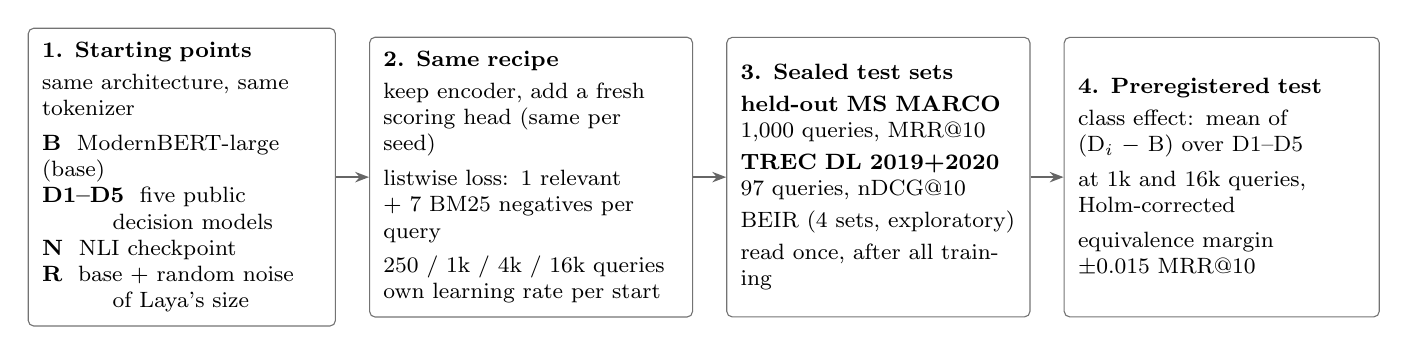
\begin{tikzpicture}[
  font=\footnotesize,
  box/.style={draw=black!55, rounded corners=2pt, align=left, inner sep=5pt, text width=#1, minimum height=3.55cm},
  head/.style={font=\footnotesize\bfseries},
  arr/.style={-{Stealth[length=5pt]}, thick, black!60},
  node distance=0.42cm
]
\node[box=3.55cm] (a) {%
  {\bfseries 1. Starting points}\\[2pt]
  same architecture, same tokenizer\\[3pt]
  \textbf{B}\ \ ModernBERT-large (base)\\
  \textbf{D1--D5}\ \ five public\\\ \ \ \ \ \ \ \ \ decision models\\
  \textbf{N}\ \ NLI checkpoint\\
  \textbf{R}\ \ base + random noise\\\ \ \ \ \ \ \ \ \ of Laya's size};
\node[box=3.75cm, right=of a] (b) {%
  {\bfseries 2. Same recipe}\\[2pt]
  keep encoder, add a fresh\\ scoring head (same per seed)\\[3pt]
  listwise loss: 1 relevant\\ + 7 BM25 negatives per query\\[3pt]
  250 / 1k / 4k / 16k queries\\
  own learning rate per start};
\node[box=3.5cm, right=of b] (c) {%
  {\bfseries 3. Sealed test sets}\\[2pt]
  \textbf{held-out MS MARCO}\\ 1{,}000 queries, MRR@10\\[2pt]
  \textbf{TREC DL 2019+2020}\\ 97 queries, nDCG@10\\[2pt]
  BEIR (4 sets, exploratory)\\[2pt]
  read once, after all training};
\node[box=3.65cm, right=of c] (d) {%
  {\bfseries 4. Preregistered test}\\[2pt]
  class effect: mean of\\ (D$_i$ $-$ B) over D1--D5\\[3pt]
  at 1k and 16k queries,\\ Holm-corrected\\[3pt]
  equivalence margin\\ $\pm$0.015 MRR@10};
\draw[arr] (a) -- (b);
\draw[arr] (b) -- (c);
\draw[arr] (c) -- (d);
\end{tikzpicture}
}
\caption{The study. Eight starting points that differ only in their weights share one recipe, each at its own learning rate, at four budgets and scored on sealed test sets.}
\label{fig:design}
\end{figure*}

\textbf{Arms} (Fig.~\ref{fig:design}, Table~\ref{tab:arms}). All arms share the ModernBERT-large architecture and tokenizer. We excluded one near-copy of Laya, detected because its weight change from the plain encoder had cosine 0.98 with Laya's. Independent checkpoints have cosines $\leq0.04$. Von is built on the NLI checkpoint (cosine 0.85). Noise (R) adds Gaussian noise to every tensor of B, scaled to the norm of Laya's change to that tensor. Only encoder weights are transferred. Every arm gets the same newly initialized ModernBERT classification head (mean pooling, dense layer, output), identical across arms for a given seed.

\begin{table}[t]
\centering
\caption{Arms. Drift: relative weight change from B. Data as stated on each model card (not verifiable).}
\label{tab:arms}
\setlength{\tabcolsep}{3pt}
\footnotesize
\begin{tabular}{@{}l l p{3.6cm} r@{}}
\toprule
Arm & Name & Training data & Drift \\
\midrule
B & ModernBERT-large & masked-language pre-training & 0 \\
D1 & Laya & undisclosed decision corpus (RL) & 4.94\% \\
D2 & Beveridge & operations documents and logs & 3.35\% \\
D3 & von & decision data incl.\ ANLI; built on N & 3.71\% \\
D4 & solvi & SQuAD 2.0, BoolQ, VitaminC & 1.40\% \\
D5 & cortex & software and security decisions & 0.68\% \\
N & NLI & GLUE and ANLI~\cite{sileo2024tasksource} & 3.11\% \\
R & Noise & B + noise of D1's per-tensor size & 4.94\% \\
\bottomrule
\end{tabular}
\end{table}

\textbf{Training.} Each query comes with its relevant passage and 7 negatives from the BM25 top-50, trained with a softmax cross-entropy loss (random guessing: $\ln 8=2.08$). We use 8 queries per step, one epoch of AdamW, 10\% warm-up and linear decay, and 256 tokens. Budgets are 250, 1k, 4k and 16k nested query samples from MS MARCO~\cite{nguyen2016msmarco} training triples, with queries from the test sets removed. Negatives come from BM25, a keyword-matching ranker~\cite{robertson2009bm25}. Each arm's learning rate is chosen on a 500-query development set from $\{1,2,4,8,16\}\times10^{-5}$ at 1k queries, and the winning run is reused as seed 0. Seeds: 3 at 1k, 2 at 250 and 4k, and at 16k 2 for B and 1 per decision arm. N and R run at 250 and 1k only.

\textbf{Test sets.} \emph{Held-out MS MARCO}: 1{,}000 unseen training-split queries, each with its positive and 20 BM25 negatives in random order (random ranking: 0.14 \ms{}). \emph{TREC DL 2019+2020}~\cite{craswell2020dl19,craswell2021dl20}: 97 queries with graded judgments, official candidates re-ranked by BM25 to the top 100, scored with \nd{}. \ms{} is the reciprocal rank of the first relevant passage within the top 10; \nd{} also credits graded relevance and position. Test scores were sealed and read once, after all training.

\textbf{Preregistered analysis.} A git tag froze the configuration and analysis code before the confirmatory runs. The class effect is the mean over D1--D5 of (D$_i-$B), each seed-averaged. Its random-effects 95\% interval is a $t$-interval over the five checkpoints. Our primary claims are at 1k and 16k, Holm-corrected, and both test sets must agree. Equivalence means a 90\% interval within $\pm$0.015 \ms{}~\cite{lakens2017equivalence}. The label is \emph{persists} (gain at 1k and 16k), \emph{fades} (gain at 1k; 16k equivalent to zero and smaller), \emph{null} (1k equivalent to zero), or otherwise \emph{inconclusive}. Secondary analyses are decision minus N and minus R at 1k, a bad-run Fisher test, and frozen-probe correlation.

\textbf{Amendments.} Before unsealing, we widened the learning-rate grid because B's best rate sat on the original grid's edge. We also added a training-failure flag (mean loss over the last tenth of steps $>0.8\ln 8$) after Laya's 16k run failed. After unsealing, we restricted the flag to runs of $\geq$100 steps. At 250 queries its ``last tenth'' is one noisy logged value, and there it had also flagged one B run. All analyses that exclude flagged runs are exploratory.

\section{Results}

\begin{figure*}[t]
\centering
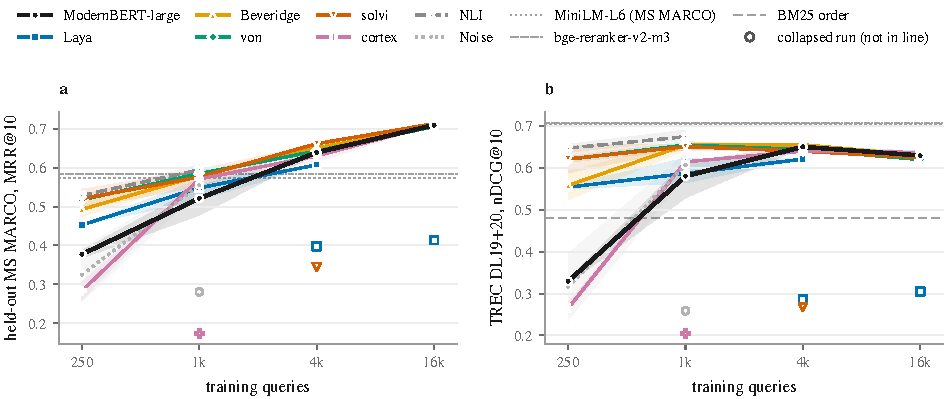
\includegraphics[width=\textwidth]{f1_learning_curves.pdf}
\caption{Learning curves on (a) held-out MS MARCO and (b) TREC DL. Lines: seed means of runs that did not collapse. Hollow markers: collapsed runs; Table~\ref{tab:main} includes them in its means, so some values differ. Horizontal lines: public rerankers and BM25 (context only).}
\label{fig:curves}
\end{figure*}

\begin{table*}[t]
\centering
\caption{Mean test score over seeds, all runs included (as preregistered). \fl: the mean includes a collapsed run. Class effect: mean of D1--D5 minus B, random-effects 95\% interval.}
\label{tab:main}
\setlength{\tabcolsep}{4.5pt}
\footnotesize
\begin{tabular}{@{}l cccc c cccc@{}}
\toprule
& \multicolumn{4}{c}{Held-out MS MARCO (\ms{})} && \multicolumn{4}{c}{TREC DL 19+20 (\nd{})} \\
\cmidrule{2-5}\cmidrule{7-10}
Arm & 250 & 1k & 4k & 16k && 250 & 1k & 4k & 16k \\
\midrule
B (ModernBERT-large) & 0.377 & 0.521 & 0.639 & 0.710 && 0.329 & 0.580 & 0.650 & 0.629 \\
D1 Laya & 0.453 & 0.548 & 0.503\fl & 0.414\fl && 0.554 & 0.587 & 0.454\fl & 0.305\fl \\
D2 Beveridge & 0.493 & 0.580 & 0.651 & 0.705 && 0.558 & 0.655 & 0.655 & 0.630 \\
D3 von & 0.517 & 0.585 & 0.643 & 0.706 && 0.620 & 0.655 & 0.644 & 0.620 \\
D4 solvi & 0.521 & 0.576 & 0.503\fl & 0.714 && 0.621 & 0.651 & 0.454\fl & 0.624 \\
D5 cortex & 0.283 & 0.439\fl & 0.631 & 0.711 && 0.265 & 0.478\fl & 0.640 & 0.637 \\
N (NLI) & 0.529 & 0.595 & -- & -- && 0.647 & 0.674 & -- & -- \\
R (Noise) & 0.324 & 0.464\fl & -- & -- && 0.316 & 0.491\fl & -- & -- \\
\midrule
Class effect & \p0.076 & \p0.025 & \m0.053 & \m0.060 && \p0.194 & \p0.024 & \m0.081 & \m0.066 \\
95\% interval & [\m.047, .199] & [\m.052, .101] & [\m.148, .042] & [\m.224, .104] && [.011, .378] & [\m.071, .120] & [\m.212, .050] & [\m.245, .113] \\
\bottomrule
\end{tabular}
\end{table*}

\begin{figure*}[t]
\centering
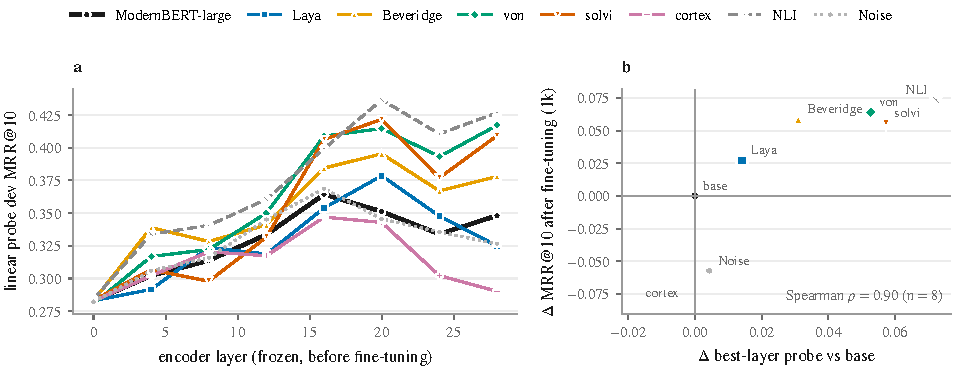
\includegraphics[width=0.9\textwidth]{f4_probes.pdf}
\caption{(a) Frozen linear probes by encoder layer, before fine-tuning. (b) Probe advantage over B against fine-tuned advantage at 1k (all runs).}
\label{fig:probes}
\end{figure*}

\textbf{Preregistered answer: inconclusive.} At small budgets most non-base arms start far ahead (Fig.~\ref{fig:curves}, Table~\ref{tab:main}). At 16k, every arm without a collapsed run averages 0.705 to 0.714 on held-out. The class effect is $+0.025$ \ms{} at 1k (95\% CI $-0.052$ to $+0.101$) and $-0.060$ at 16k ($-0.224$ to $+0.104$), with similar DL values. Both Holm $p$-values are 0.74 and neither budget is equivalent to zero, so the preregistered label is \textbf{inconclusive}. B needs about 33\% more queries to match the decision class at 1k.

\textbf{Why: collapsed runs.} In five of the 59 analysed runs, the training loss stayed near the random-guess level: Laya at 16k and at 4k (seed 1), solvi at 4k (seed 1), cortex at 1k (seed 2) and Noise at 1k (seed 2). These runs scored 0.17 to 0.41 \ms{}, against 0.54 to 0.66 for the same arms' other runs at that budget. All five ran above B's rate, two of them at the very budget where the rate was chosen. Laya's loss at $1.6\times10^{-4}$ falls, climbs back towards chance and stays near 1.7; at B's rate the same checkpoint trains normally (Fig.~\ref{fig:loss}). In the learning-rate search B fails at $1.6\times10^{-4}$ (0.354 dev \ms{}), where Laya, Beveridge and solvi still score $\geq$0.556. B never trained at those rates in a confirmatory run, so we cannot separate checkpoint fragility from rate fragility. The preregistered bad-run test (a run $>$0.05 \ms{} below its arm's median) finds no difference: 3/40 decision vs.\ 1/9 base runs, Fisher $p=0.57$.

\begin{figure}[t]
\centering
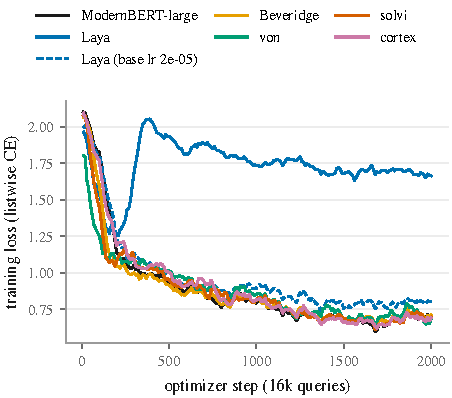
\includegraphics[width=0.92\columnwidth]{fa2_loss.pdf}
\caption{Training loss at 16k queries. Laya at its selected rate collapses; at B's rate (dashed) it trains normally.}
\label{fig:loss}
\end{figure}

\textbf{Without collapses: a head start that fades} (exploratory, Table~\ref{tab:sens}). Excluding flagged runs, the decision class leads by $+0.051$ \ms{} and $+0.052$ \nd{} at 1k. Every checkpoint is ahead, and so is the class within each seed. The lead is zero at 4k and equivalent to zero at 16k, so the preregistered rule returns \textbf{fades}. The size is uncertain, though. B's three 1k seeds vary widely (0.478 to 0.553), and also dropping B's weakest gives $+0.029$, with DL no longer significant. We read the head start as $+0.03$ to $+0.05$ \ms{}.

\begin{table}[t]
\centering
\caption{Class effect, random-effects 95\% interval. Rows below the first are exploratory.}
\label{tab:sens}
\setlength{\tabcolsep}{2.5pt}
\resizebox{\columnwidth}{!}{%
\begin{tabular}{@{}l l c c@{}}
\toprule
Analysis & & Held-out \ms{} & DL \nd{} \\
\midrule
Preregistered & 1k & \p0.025 [\m0.052, \p0.101] & \p0.024 [\m0.071, \p0.120] \\
Excl.\ collapsed runs & 1k & \p0.051 [\p0.033, \p0.069] & \p0.052 [\p0.014, \p0.090] \\
& 4k & \m0.000 [\m0.027, \p0.026] & \m0.010 [\m0.025, \p0.005] \\
& 16k$^{a}$ & \m0.001 [\m0.007, \p0.005] & \m0.002 [\m0.013, \p0.010] \\
\quad + excl.\ B's weakest seed & 1k & \p0.029 [\p0.012, \p0.047] & \p0.026 [\m0.012, \p0.064] \\
\bottomrule
\multicolumn{4}{@{}l}{\footnotesize $^{a}$Four checkpoints: Laya's only 16k run collapsed.}
\end{tabular}}
\end{table}

\textbf{Not about decisions} (Table~\ref{tab:spec}). With all runs, the decision class trails NLI at 1k by 0.049 \ms{} and beats Noise by 0.082 (both preregistered contrasts Holm $p<0.001$). The Noise margin, however, comes from its one collapsed run. Excluding collapsed runs symmetrically, Noise itself is $+0.034$ ahead of B and the decision class leads it by only $+0.017$, while NLI still leads the decision class. Von, which is decision training on top of the NLI checkpoint, is slightly below NLI. At B's shared rate (one seed), no decision head start is detectable ($-0.001$, 95\% CI $\pm0.04$), while NLI keeps $+0.029$.

\begin{table}[t]
\centering
\caption{Contrasts at 1k, held-out \ms{} (query-bootstrap 95\% intervals).}
\label{tab:spec}
\setlength{\tabcolsep}{3pt}
\resizebox{\columnwidth}{!}{%
\begin{tabular}{@{}l c c@{}}
\toprule
Contrast & All runs (prereg.) & Collapsed excl.\ (explor.) \\
\midrule
Decision $-$ B & \p0.025 [\p0.012, \p0.037] & \p0.051 [\p0.039, \p0.064] \\
NLI $-$ B & \p0.074 [\p0.058, \p0.090] & \p0.074 [\p0.058, \p0.090] \\
Noise $-$ B & \m0.057 [\m0.071, \m0.044] & \p0.034 [\p0.021, \p0.048] \\
Decision $-$ NLI & \m0.049 [\m0.059, \m0.039] & \m0.023 [\m0.033, \m0.012] \\
Decision $-$ Noise & \p0.082 [\p0.070, \p0.094] & \p0.017 [\p0.005, \p0.029] \\
\bottomrule
\end{tabular}}
\end{table}

\textbf{The frozen encoder already knows.} A logistic probe on frozen mean-pooled features, fitted on 1k queries, measures how much relevance signal each starting point holds before fine-tuning (Fig.~\ref{fig:probes}). Across the eight arms, the probe's advantage over B predicts the fine-tuned advantage at 1k (Spearman $\rho=0.90$, exact $p=0.005$; preregistered, descriptive; $\rho=0.76$ without collapsed runs). NLI, solvi and von carry the most signal, and cortex and Noise no more than B.


\textbf{Transfer and cost.} On four BEIR sets~\cite{thakur2021beir} (4k and 16k, seed 0, exploratory), no starting point is consistently better, and more MS MARCO data does not reliably help. All 95 training runs took 4.1 GPU-hours on one RTX 3090, plus 1.4 for scoring.

\section{Discussion and Limitations}

For practitioners, the starting point did not matter here once a few thousand labelled queries were available. With fewer, an NLI checkpoint was the best starting point. The habits that mattered most were searching each checkpoint's learning rate, checking it on more than one seed, and watching the training loss for collapse. A frozen probe, which costs minutes, ranked the starting points much as fine-tuning did. Our conclusions are scoped to one backbone and five community checkpoints of unverifiable provenance. The analyses without collapsed runs were chosen after unsealing. N and R are single checkpoints trained only up to 1k. And B never ran at the higher rates that the other arms chose. The repository documents every analysis, figure and amendment.

\section*{Acknowledgment}
An AI assistant (Claude, Anthropic) helped write code and draft parts of this text; the authors checked all numbers and take responsibility for the content.

\bibliographystyle{IEEEtran}
\bibliography{../refs}

\end{document}
